% Chapter Template

\chapter{Scenario} % Main chapter title

\label{Chapter3} % Change X to a consecutive number; for referencing this chapter elsewhere, use \ref{ChapterX}

\textit{In questo capitolo facciamo un introduzione su quelloo he è lo scenario che stiamo considerando per il nostro lavoro, ovvero 
quello delle comunicazioni satellitare e di quali sono le attuali tecnologie utilizzate per realizzarle.}
\todo{Riformula meglio}

%----------------------------------------------------------------------------------------
%	SECTION 1
%----------------------------------------------------------------------------------------

\section{Comunicazioni Satelliari}


Le comunicazioni satellitari sono una fondamenta delle infrastrutture moderne, abilitando una vasta gamma di servizi.
Negli ultimi decenni, con l'aumento della domanda di connettività globale e l'espansione delle reti di comunicazione, i satelliti sono diventati strumenti essenziali per garantire una copertura estesa.
L'emergere delle costellazioni di satelliti in orbita bassa (LEO - Low Earth Orbit) sta cambiando il paradigma delle comunicazioni satellitari, offrendo vantaggi significativi rispetto ai satelliti geostazionari (GEO), un confronto tra la differenza di distanze è mostrato in \textit{Figura \ref{fig:orbite}}. 
%Mentre i satelliti GEO forniscono una copertura stabile, i satelliti LEO consentono Round Time Trip (RTT) notevolmente ridotti e una maggiore flessibilità, rendendoli ideali per applicazioni ad alta velocità come la trasmissione dati in tempo reale e la connettività Internet globale.
\todo{Scrivere meglio questa parte finale}
Questo cambio di paradigma insieme al quantum computer hanno portato diversi enti, tra cui l'Agenzia Spaziale Europea (ESA), ad affrontare nuove sfide.

\begin{figure}[h!]
    \centering
    \begin{tikzpicture}
        % Definizione dei colori per le orbite
        \definecolor{leo}{gray}{0.2}    % Grigio scuro
        \definecolor{geo}{gray}{0.1}% Grigio molto scuro
        \definecolor{terra}{HTML}{008F39}
        \node at (-4.8, 0) [color=geo]{GEO};
        \node at (3.5, 0) [color=leo]{LEO};
        \node at (0, 0) {Terra};
        
        \draw[thick, dashed, geo] (0,0) circle (4.2cm);
        \draw[thick, dashed, leo] (0,0) circle (3cm);
        \filldraw[fill=mare,] (0,0) circle (2.2cm);

        \path[draw, decoration={text along path, text={$2.000km$}, text align=center}, decorate] (0,0) (180:2.8cm) arc (180:360:2.8cm);
        \path[draw, decoration={text along path, text={$36.000km$}, text align=center}, decorate] (0,0) (180:4cm) arc (180:360:4cm);

        \node at (-2.5,2) {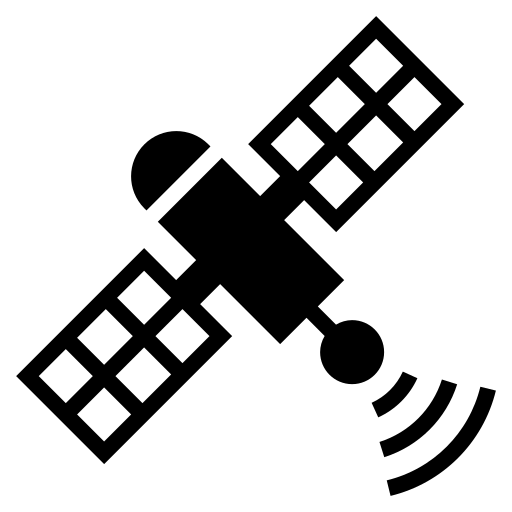
\includegraphics[width=1cm]{Figures/satellite.png}}; % Sostituisci 'your_image.png' con il percorso della tua immagine
        \node at (3.2,3) {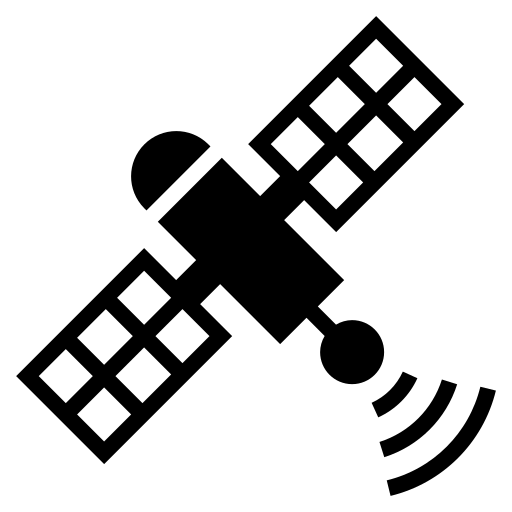
\includegraphics[width=1cm, angle=270]{Figures/satellite.png}}; % Sostituisci 'your_image.png' con il percorso della tua immagine
        \node at (0.2,0.5) {
\includegraphics[width=3cm ]{Figures/europe.png}}; % Sostituisci 'your_image.png' con il percorso della tua immagine

        \node[cloud, cloud puffs=15.7, cloud ignores aspect, minimum width=1.5cm, minimum height=0.5cm, align=center, fill=white, draw] (cloud) at (-2, 0) {};
        \node[cloud, cloud puffs=15.7, cloud ignores aspect, minimum width=1.5cm, minimum height=0.5cm, align=center, fill=white, draw] (cloud) at (2, -0.5) {};

    \end{tikzpicture}
    \caption{Orbite dei satelliti}
    \label{fig:orbite}
\end{figure}

\subsection{Limitazioni}

L'ambiente spaziale, caratterizzato da radiazioni intense, temperature estreme e lunghi periodi senza manutenzione, pone sfide significative in termini di progettazione e operatività dell'hardware e del software.
Tra i principali vincoli per l'hardware satellitare troviamo:

\begin{itemize}
    \item \textit{Resistenza alle radiazioni}: i componenti elettronici devono essere progettati per resistere all'esposizione costante alle radiazioni spaziali
    \item \textit{Basso consumo energetico}: l'energia disponibile per le operazioni\\ computazionali è limitata, quindi si usano processori a basso consumo e ad alta efficienza energetica, sacrificando potenza di calcolo.
    \item \textit{Elaborazione in tempo reale}: per alcune tipologie di servizi è necessario che il processamento avvenga in tempo reale.
    \item \textit{Compattezza}: a causa dello spazio limitato a bordo di un satellite, i componenti hardware devono essere progettati in modo estremamente compatto.
\end{itemize}

\noindent
L'hardware limitato ha un impatto diretto sullo sviluppo del software per i satelliti. 
Rispetto al un contesto terrestre, dove le risorse computazionali sono abbondanti, il software per i satelliti deve essere ottimizzato per funzionare su processori con bassa potenza di calcolo, limitato parallelismo e memoria ridotta. 
Le principali sfide per gli sviluppatori sono:

\begin{itemize}
    \item \textit{Semplicità e ottimizzazione}: gli algoritmi devono essere semplici e ottimizzati per funzionare su hardware con risorse limitate.
    \item \textit{Parallelismo limitato}: non è possibile sfruttare un alto grado di parallelismo computazionale. Le operazioni devono essere eseguite in modo lineare o con limitato parallelismo, aumentando la complessità della progettazione.
    \item \textit{Affidabilità assoluta}: il software deve essere robusto, sicuro e testato ampiamente in modo tale che possibile errori non abbiano conseguenza catastrofiche.
\end{itemize}

\noindent
Particolare attenzione va posta sulle implementazinoni crittografiche, dato che in questo contesto è essenziale riuscire a bilanciare sicurezza e prestazioni
Occorre ridurre al minimo l'impatto sulle risorse in modo tale che gli algoritmi di crittografia non possano compromettere l'efficienza operativa del satellite.

\subsection{Stato Attuale}

Per capire quale è la differenza in termini di hardware e software rispetto a quelli a cui siamo abiutati 
introduciamo quelli che sono gli attuali standard impiegati in questo settore.

\begin{itemize}
    \item Tra i processori utilizzati abbiamo \textit{LEON3}, un processore open-source basato sull'architettura SPARC, progettato dall'ESA. 
    \item ESA Power Interface Standard (ECSS-E-ST-20C): definisce come deve avvenire la distribuituzione dell'alimentazione elettrica all'interno dei satelliti.
    \item Cubesat Standard: definisce dimensioni compatte modulari (10x10x10 cm per 1U) per ridurre i costi e semplificare il lancio e la costruzione dei satelliti.
    \item Triple Modular Redundancy (TMR): nei sistemi critici spaziali si utilizza la ridondanza tripla modulare, per garantire l'affidabilità dei risultati tramite sistemi di voting.
\end{itemize}
\noindent
Il sistema operativo utilizzato in queste applicazioni è RTEMS (Real-Time Executive for Multiprocessor Systems) che le caratteristiche di essere open-source, real-time e basato su GNU/Linux.
\todo{se si trova riportare qualche riferimento}

%-----------------------------------
%	SECTION 2
%-----------------------------------
\subsection{Sfide}
\todo{Scrivere bene quelle che sono le problematiche e come intendiamo affrontarle}
Come detto con il post-quantum tutto diventa più pesante e più lento, in generale.
Andiamo a caratterizzare quella che è l'impronta computazionale degli algoritmi nel caso desktop rispetto a quella di quelli classici per 
vederne le differenze, se queste sono molto evidenti già nel caso simulato allora non ha neanche senso andarle a considerare in un'ambiente
ancora più limitato.

Considerereremo nelle nostre prove quelli che sono i finalisti del processo di standardizzazione del NIST, in particolare la loro implementazione
forniata da \textbf{open quantum safe} (oqs). Vedremo il loro utilizzo nell'implementazione del protocollo IKEv2, Strongswan.

\section{Benchmarking}
Come abbiamo effettuato il benchmarking
Quindi introdurre tutta la parte di scripting e di automatizazione tramite docker

\section{Tuttavia}

Notiamo che non ci sono enormi differenze in termini di tempi ma tuttavia notiamo una notevole differenza
in termini della dimensione. E in contesto di questo tipo non è auspicabile

Cercando di trovare possibili soluzioni, ci siamo imbattuti su quello che è minimal IKE ovvero
una versione di IKE applicabile in scenari soggetti a constraint di risorse simili a quelli presenti nello spazio.

Riguardo a questo non esistono implementazioni, per questo motivo siamo passati a provare a dare un'implementazione di quest'ultimo
In modo tale che rappresenti un punto di inizio per questo scenario

Di questo trattiamo nel prossimo capitolo

%-----------------------------------
%	SECTION 3
%-----------------------------------


